\documentclass[12pt, conference, compsoc, onecolumn]{IEEEtran}
\usepackage{graphicx}
\usepackage{listings}
\usepackage{array, float}
\usepackage[colorlinks=true]{hyperref}
\usepackage[style=numeric,backend=bibtex]{biblatex}
\graphicspath{ {./figures/} }
\addbibresource{refs.bib}

\lstdefinestyle{model_arch}{
	backgroundcolor=\color{white},   
	basicstyle=\ttfamily,
	breaklines=true,
	showstringspaces=false,
	frame=single, % This adds a box around all sides of the snippet
	rulecolor=\color{black}, % You can specify the color of the box
}

\begin{document}
	\title{ECE1512 - Digital Image Processing and Applications - Project B}
	\author{Swapnil Patel - 999728870 - \today}
	
	\author{\IEEEauthorblockN{Swapnil Patel}
		\IEEEauthorblockA{
			University of Toronto\\
			swap.patel@mail.utoronto.ca\\
			Code: \href{https://github.com/Swapnil949/ECE1512\_2024F\_ProjectRepo\_SwapnilPatel}{Swapnil949/ECE1512\_2024F\_ProjectRepo\_SwapnilPatel}
	}}
	
	\maketitle
	
	\section{State Space Models (SSMs) [Mamba: Linear-Time Sequence Modeling with Selective State Spaces]}
	In this section, Mamba, as introduced in the paper "Mamba: Linear-Time Sequence Modeling with Selective State Spaces" \cite{gu2024mamba}, is discussed. Mamba is a novel sequence modeling architecture that leverages Selective State Space Models (SSMs) to address the computational inefficiencies of Transformers while maintaining their ability to perform complex reasoning. The architecture introduces input-dependent dynamics in SSM parameters, enabling selective propagation or forgetting of information along sequences.
	
	This work represents a significant step forward in designing models that combine efficiency and performance, achieving linear scaling in sequence length and demonstrating up to 5× higher inference throughput compared to Transformers. Mamba eliminates the need for attention or MLP blocks, offering a simplified design suitable for multimodal tasks. It achieves state-of-the-art results across various domains, including language, audio, and genomics, and matches the performance of Transformers twice its size in language modeling tasks.
	
	Mamba is designed to solve the computational inefficiency and scalability issues of Transformers, particularly for handling long sequence data across various modalities (e.g., language, audio, and genomics). The primary challenges that Mamba addresses are:
	
	\subsubsection*{Inefficiency of Self-Attention in Transformers}
	\begin{itemize}
		\item \textbf{Quadratic Complexity:} The self-attention mechanism in Transformers scales quadratically with sequence length, making it computationally expensive and memory-intensive for long sequences \cite{vaswani2023attentionneed}.
		\item \textbf{Limited Context:} Transformers can only process a finite context window efficiently, which limits their ability to model long-range dependencies.
	\end{itemize}
	
	\subsubsection*{Limitations of Existing Efficient Architectures}
	\begin{itemize}
		\item Several subquadratic-time models (e.g., linear attention \cite{katharopoulos2020transformersrnnsfastautoregressive}, gated convolution \cite{rao2022hornetefficienthighorderspatial}, recurrent models \cite{bulatov2022recurrentmemorytransformer}, and structured state space models \cite{gu2022efficientlymodelinglongsequences}) have been proposed to improve efficiency. However they have their own drawbacks. 
		\begin{itemize}
			\item They often fail to match the performance of Transformers, especially in discrete and information-dense data such as natural language.
			\item They lack content-based reasoning capabilities, which are crucial for tasks like language modeling and in-context learning.
			
		\end{itemize}
		
	\end{itemize}
	
	\subsection{Mamba Architecture}
	\begin{figure}[H]
		\centering
		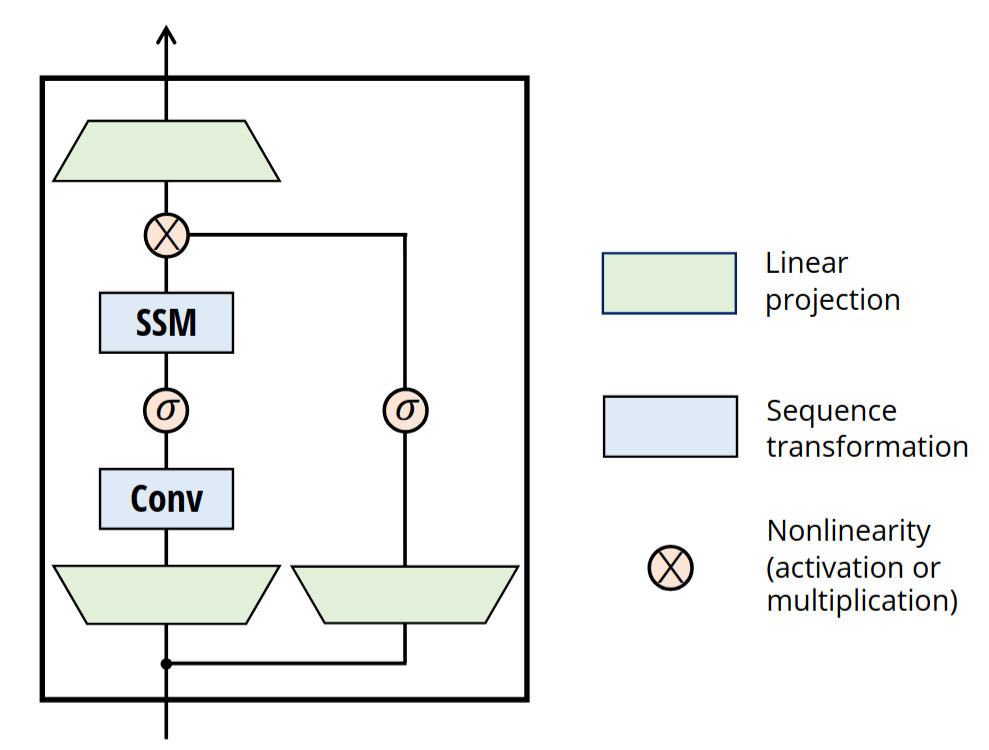
\includegraphics[width=0.48\textwidth]{figures/mamba_arch.png}
		\caption{Mamba Architecture\cite{gu2024mamba}}
		\label{fig:mamba_arch}
	\end{figure}
	
	
	
	\subsection{MambaVision}
	\begin{figure}[H]
		\centering
		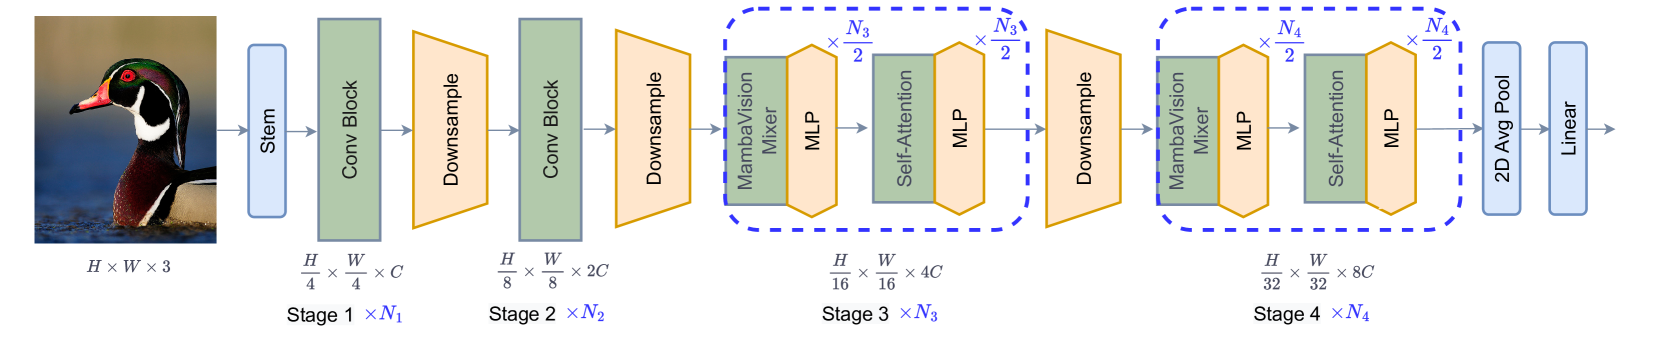
\includegraphics[width=0.99\textwidth]{figures/mambavision_arch.png}
		\caption{Mambavision Architecture\cite{hatamizadeh2024mambavision}}
		\label{fig:mambavision_arch}
	\end{figure}
		
	\begin{figure}[H]
		\centering
		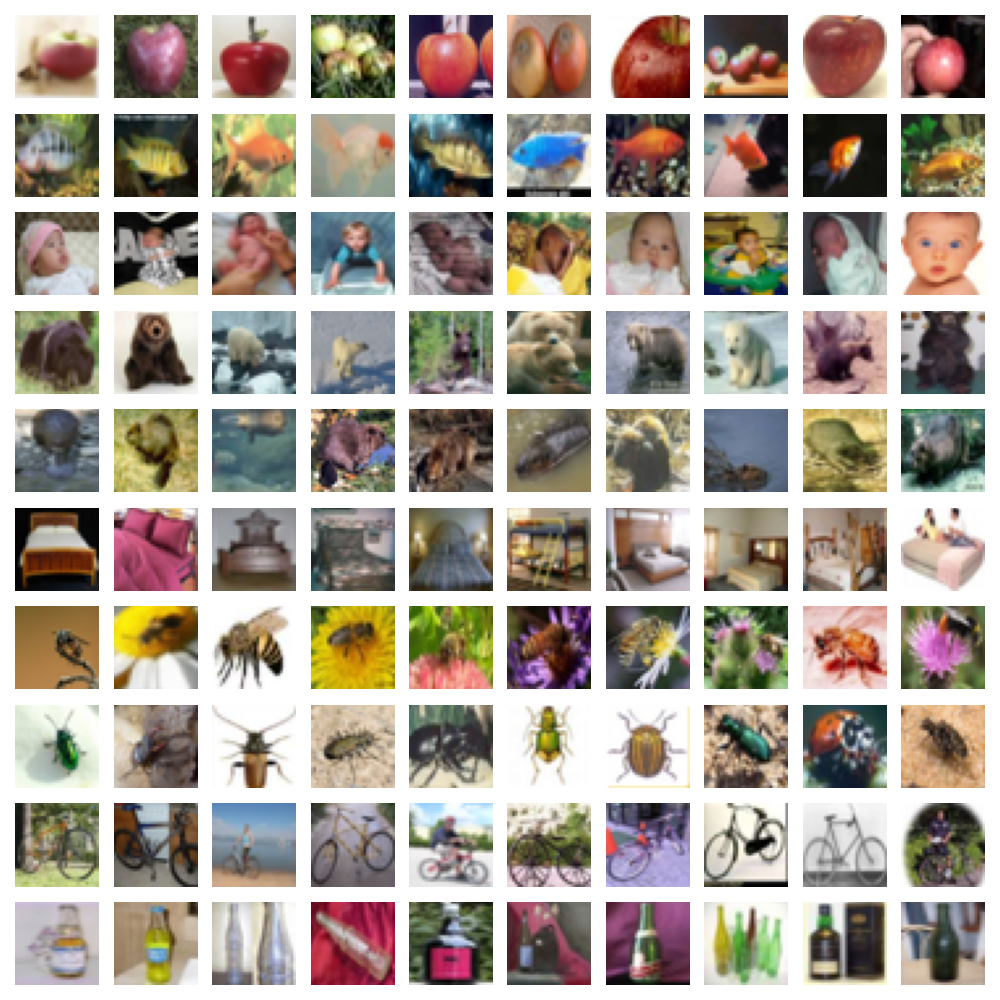
\includegraphics[width=0.75\textwidth]{figures/cifar100_sample.png}
		\caption{Sample of CIFAR100 Dataset\cite{Krizhevsky09cifar100}}
		\label{fig:cifar100}
	\end{figure}
	
	\newpage
	\section{LLaVA - Large Language and Vision Assistant}
	
	In this section, LLaVA (Large Language and Vision Assistant), as presented in the paper "Visual Instruction Tuning" \cite{liu2023llava}, is discussed. LLaVA is an end-to-end trained multimodal AI system that connects a vision encoder with a large language model (LLM) to interpret and follow human instructions involving both visual and linguistic contexts. The work in this paper represents the first attempt to use language-only GPT-4 to generate multimodal language-image instruction-following data, enabling instruction tuning for multimodal tasks.
	
	The paper demonstrates that LLaVA achieves remarkable capabilities in multimodal chat, often exhibiting behaviors similar to multimodal GPT-4 on unseen images and instructions. Evaluations show an 85.1\% relative score compared to GPT-4 on a synthetic multimodal instruction-following dataset. Furthermore, when fine-tuned on ScienceQA, LLaVA achieves a new state-of-the-art accuracy of 92.53\%, highlighting its effectiveness in reasoning and answering visual and textual queries. To facilitate further research, the authors release the GPT-4-generated visual instruction tuning data, their model, and associated codebase to the public.
	
	\subsection{LLaVA Architecture}
	\begin{figure}[H]
		\centering
		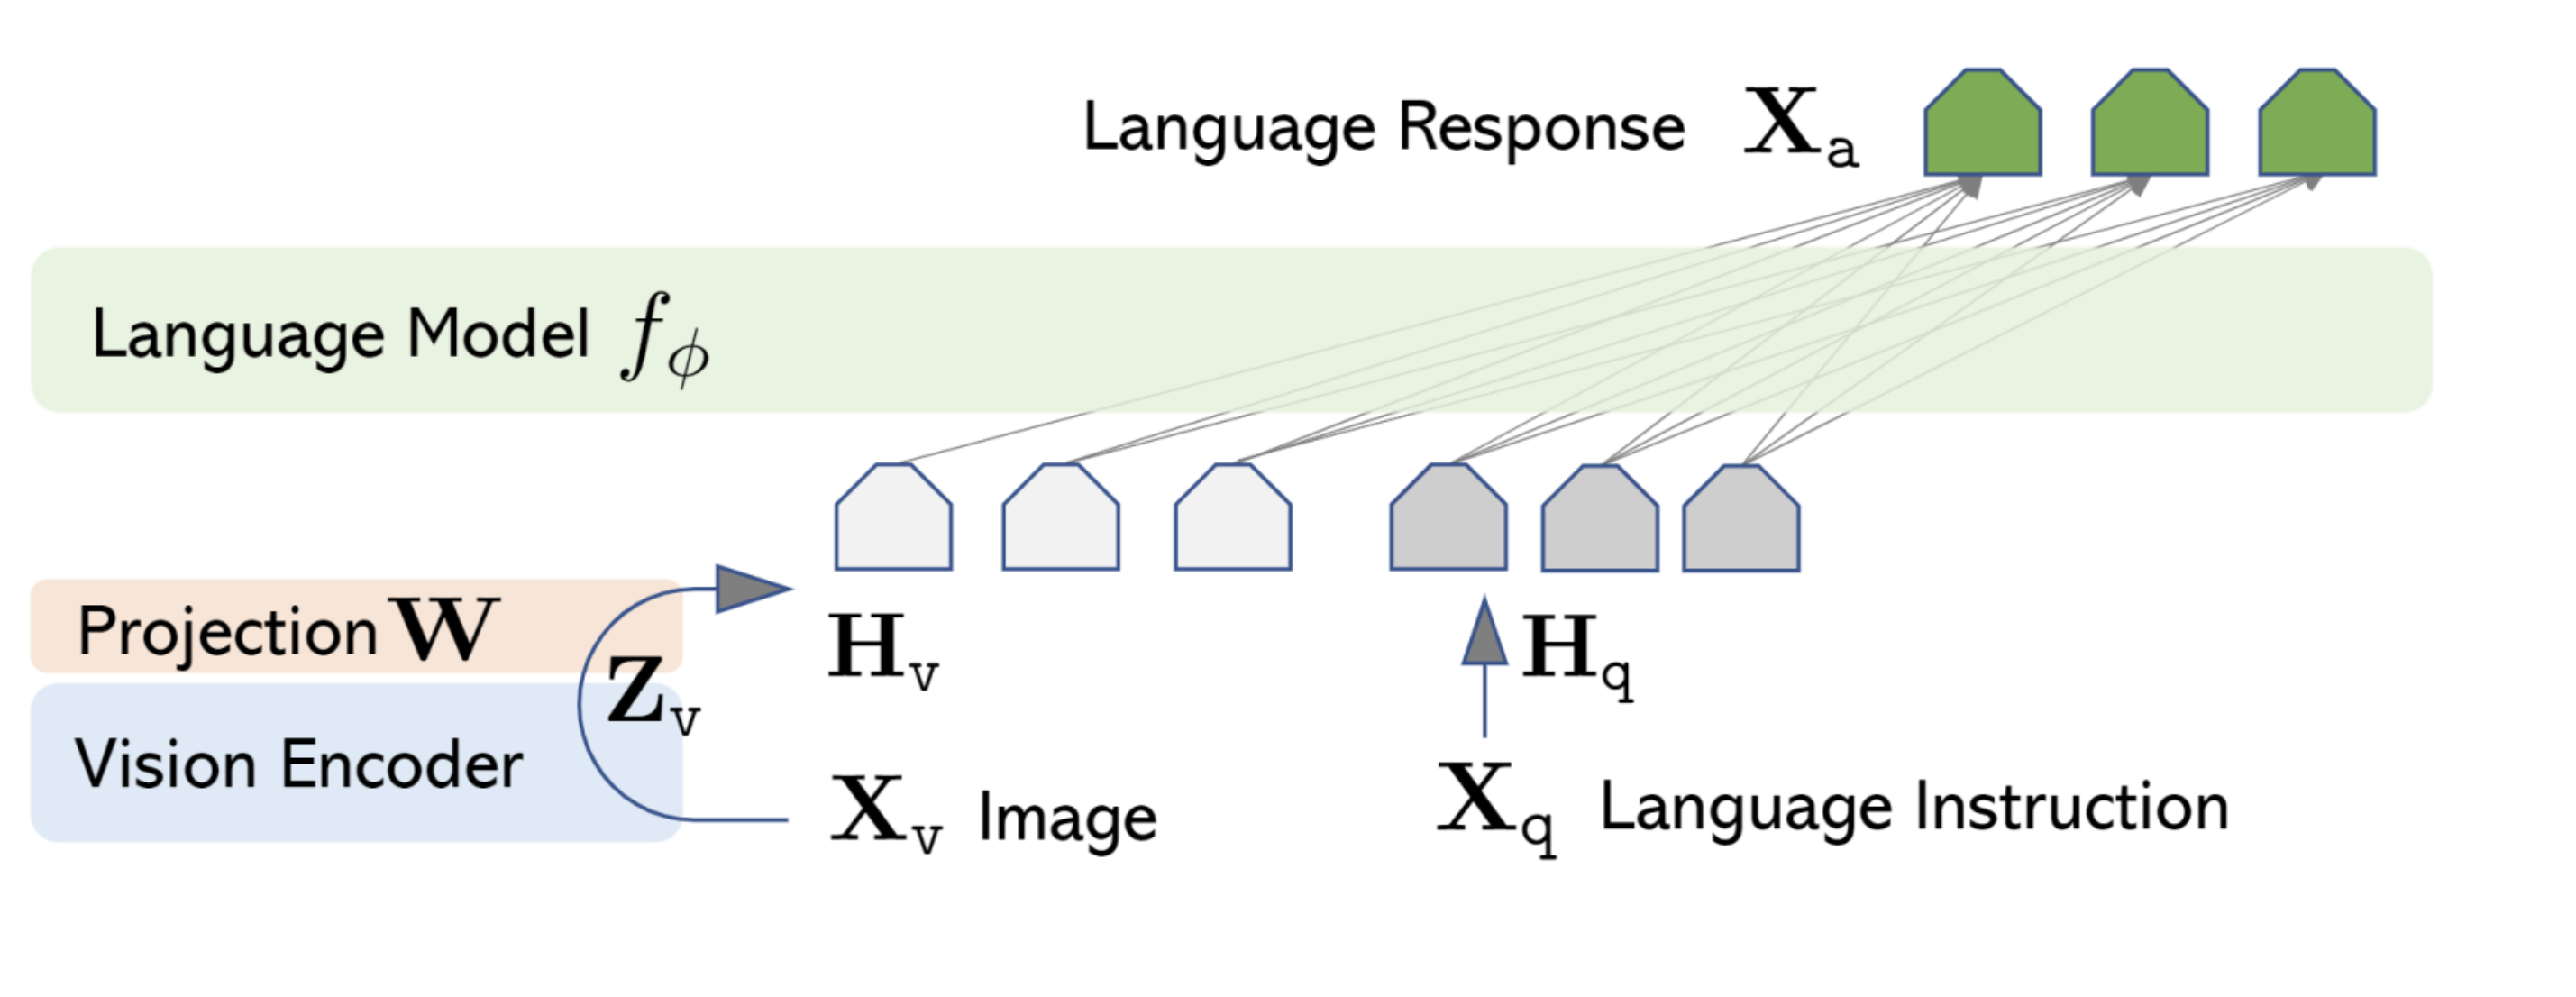
\includegraphics[width=0.75\textwidth]{figures/conceptual-diagram-of-llava.png}
		\caption{LLaVA Architecture \cite{liu2023llava}}
		\label{fig:llava_arch}
	\end{figure}
	
	The LLaVA (Large Language and Vision Assistant) model architecture is designed to integrate visual and linguistic modalities to enable advanced multimodal understanding. Its structure consists of several key components, which work together to process both image and text inputs, generating coherent and context-aware responses.
	\subsubsection*{Vision Encoder} 
	At the foundation of the architecture is the Vision Encoder, which processes the input image $X_v$. This encoder (e.g., CLIP) transforms the raw image data into a high-dimensional feature representation $H_v$. These features encapsulate the visual information in a format suitable for downstream processing.
	
	\subsubsection*{Projection Layer} 
	The Projection Layer serves as a critical bridge between the Vision Encoder and the Language Model. It applies a projection matrix $W$ to convert the feature representations $H_v$ into a format $Z_v$ that is compatible with the language model's embedding space. This alignment ensures seamless integration of visual data with textual data for joint processing.
	
	\subsubsection*{Language Instruction Input}
	Alongside the visual input, the model receives a Language Instruction input $X_q$, which represents the textual task or query. This input is processed by the language model to generate its own feature representation $H_q$, encapsulating the semantic meaning of the query.
	
	\subsubsection*{Language Model}
	At the core of the architecture is the Language Model $f_\phi$, which is a pre-trained large language model (e.g., Vicuna). This model takes both the projected visual features $Z_v$ and the linguistic features $H_q$ as input, integrating them to produce a unified understanding of the multimodal context.
	
	\subsubsection*{Output Generation}
	The final output, $X_a$, is a language-based response that incorporates information from both the visual and textual inputs. This response can range from answering specific questions about an image to providing detailed descriptions or engaging in complex reasoning tasks that require a multimodal perspective.
	
	
	\section*{References}
	\addcontentsline{toc}{section}{\protect\numberline{}References}
	\nocite{*}
	\printbibliography[heading=none]
	
	%	\onecolumn
	%	\section*{Appendix}
	%	\addcontentsline{toc}{section}{\protect\numberline{}Appendix}
	
	
\end{document}